\chapter{Introducción}
Las imágenes de radar de apertura sintética (SAR, por sus siglas en inglés) son una técnica de adquisición remota de datos que utiliza ondas de radio para generar imágenes de alta resolución de la superficie terrestre, y representan una valiosa fuente de información para su análisis. Su principal ventaja radica en su capacidad para adquirir datos de calidad independientemente de las condiciones climáticas o de iluminación, superando así las limitaciones de otras tecnologías de observación remota, como las imágenes ópticas. Gracias a esto, las imágenes SAR son ampliamente utilizadas en aplicaciones que van desde la vigilancia ambiental hasta la detección de cambios en el terreno y el monitoreo de desastres naturales.

Sin embargo, una de las principales desventajas de este tipo de imágenes es la presencia de ruido \emph{speckle}. A diferencia de otros tipos de ruido más convencionales, el \emph{speckle} no es aditivo ni sigue una distribución gaussiana, lo que dificulta significativamente su modelado y eliminación. Es un ruido multiplicativo, lo cual implica que su efecto depende de la intensidad de cada pixel. Este fenómeno surge como consecuencia de la interferencia coherente entre las múltiples señales reflejadas por los objetos en la superficie terrestre, generando patrones granulosos que afectan la calidad visual de las imágenes y dificultan su posterior análisis.

A lo largo de los años, se han propuesto diversas técnicas para la mitigación del ruido \emph{speckle}. En particular, el avance de las técnicas de aprendizaje profundo (\textit{Deep Learning}) ha abierto nuevas posibilidades en esta área. En la actualidad, muchas de las soluciones más prometedoras se basan en arquitecturas de redes neuronales convolucionales (CNNs) y, en menor medida, en modelos de autoencoders. Estas redes se entrenan en un entorno supervisado, donde se requiere disponer de pares de imágenes: una con ruido y su correspondiente versión libre de ruido. El objetivo del modelo es aprender a mapear las imágenes SAR ruidosas hacia representaciones más limpias, preservando al mismo tiempo las características estructurales y texturales de la escena.

No obstante, este enfoque presenta un desafío importante: en la práctica no se dispone de imágenes SAR reales sin ruido, lo que obliga a recurrir a técnicas de simulación para generar versiones artificiales del ruido \emph{speckle} sobre imágenes limpias. Esto a su vez implica la creación de modelos capaces de describir y simular el ruido \emph{speckle} de manera precisa. A partir de estas simulaciones se construyen los conjuntos de datos necesarios para entrenar los modelos de \emph{deep learning}.

Existen múltiples trabajos en la literatura que aplican este enfoque, pero la mayoría se basa en métodos de generación de ruido que resultan limitados. Por un lado, algunos utilizan modelos obsoletos o simplificados que no reflejan adecuadamente la complejidad estadística del ruido \emph{speckle} real. Por otro lado, hay enfoques que están diseñados específicamente para ciertos tipos de superficie (como vegetación, cuerpos de agua o zonas urbanas) y no generalizan bien a otros escenarios.

La distribución \( \mathcal{G}_I^0 \) es altamente flexible y robusta, y permite representar de manera más realista la variabilidad del ruido \emph{speckle} en distintos tipos de terreno. Incorporarla en los procesos de simulación para el entrenamiento de modelos de \emph{deep learning} es algo que en la literatura aún no se ha explorado y podría mejorar significativamente la calidad de los modelos elimnación de ruido, ampliando su aplicabilidad y capacidad de generalización.

\section{Imágenes SAR y la generación de ruido \emph{speckle}}

Las imágenes SAR se obtienen mediante sensores activos que emiten ondas de radio y miden la señal reflejada por la superficie terrestre. Se generan a partir de la información de fase y amplitud de las ondas reflejadas, lo cual permite construir imágenes de alta resolución espacial. En la Figura \ref{fig:imagenes_sar_ruido} se ven dos ejemplos de imágenes reales, de la ciudad de San Francisco, CA, USA (Figura~\ref{Sanfran}) y de los alredededores de la ciudad de Mucnich, Alemania (Figura~\ref{Munich}).

\begin{figure}[htbp]
    \centering
    \begin{subfigure}[b]{0.48\textwidth}
        \centering
        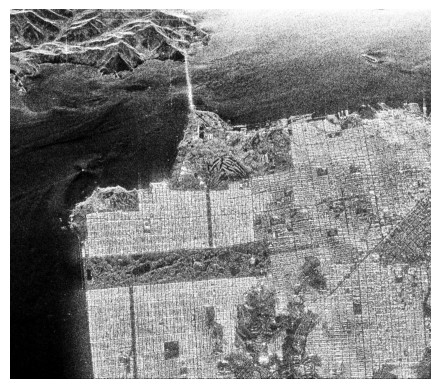
\includegraphics[height=6.9cm]{Images/sar_sanfran.jpg}
        \caption{Bahía de San Francisco, CA, EEUU.}
        \label{Sanfran}
    \end{subfigure}
    \hfill
    \begin{subfigure}[b]{0.48\textwidth}
        \centering
        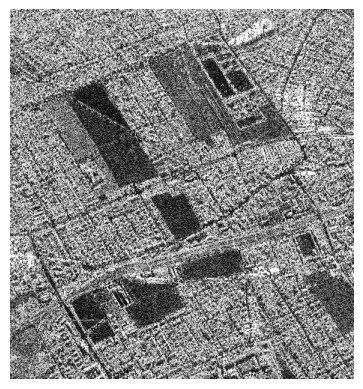
\includegraphics[height=6.9cm]{Images/sar_munich.jpg}
        \caption{Ciudad de Múnich, Alemania.}
        \label{Munich}
    \end{subfigure}
    \caption{Ejemplo de imágenes SAR con ruido reales.}
    \label{fig:imagenes_sar_ruido}
\end{figure}

Una de las características distintivas del ruido en imágenes SAR es su naturaleza multiplicativa, a diferencia del ruido aditivo común en imágenes ópticas. Esto significa que el ruido no se suma a la señal, sino que se multiplica por ella, amplificándose en las zonas de mayor intensidad (mayor retorno de señal) y siendo menos notable en las regiones más oscuras. Como consecuencia, este tipo de ruido genera una textura granular que dificulta la posterior interpretación de la imagen.

La señal que regresa al sensor después de interactuar con la superficie terrestre es conocida como backscatter, y es la base para construir la intensidad de píxeles en la imagen. El valor del backscatter varía según propiedades físicas de la superficie, como su rugosidad, el contenido de humedad, el ángulo de incidencia del radar y la polarización utilizada. En general, superficies rugosas o con estructuras complejas, como áreas urbanas o vegetación densa, generan un mayor ruido \emph{speckle}, mientras que superficies lisas como cuerpos de agua desvían la señal en otras direcciones y aparecen más oscuras en la imagen.

En el ámbito de las imágenes SAR, el número de \emph{looks} hace referencia al grado de reducción de \emph{speckle} que se logra mediante el procesamiento multi-\emph{look}, el cual promedia múltiples observaciones independientes (o \emph{looks}) de una misma área. Estas observaciones pueden generarse dividiendo la señal recibida en sub-bandas espectrales o espaciales, y su combinación permite suavizar la variabilidad aleatoria introducida por el ruido \emph{speckle}, especialmente en regiones homogéneas. A medida que aumenta el número de \emph{looks}, el ruido se reduce de forma significativa, pero también puede producirse una pérdida de resolución espacial. Por este motivo, se busca un equilibrio entre la mejora de la imagen y la preservación de sus detalles estructurales. Para cuantificar este balance, se utiliza el concepto de Número Equivalente de \emph{Looks} (ENL por sus siglas en inglés), una medida estadística que estima la relación entre el cuadrado de la media y la varianza de la intensidad en una región homogénea. valor de ENL alto indica una imagen más homogénea y con menor ruido, mientras que un valor de ENL bajo sugiere una mayor presencia de \emph{speckle}. Este parámetro es ampliamente utilizado para evaluar la calidad de las imágenes SAR procesadas y comparar distintos métodos de reducción de ruido.

Uno de los métodos clásicos para generar imágenes sintéticas con ruido \emph{speckle} es el uso de modelos estadísticos, como la distribución $\Gamma$. Otra alternativa es la distribución de Rayleigh, aunque esta última solo es efectiva para superficies de pastura. Hay trabajos, como el de Wang et al. \cite{wang2017sar}, que aplican sus propios enfoques estadísticos para simular el ruido, conociendo previamente algunas características del mismo. Además de los modelos estadísticos, también existen modelos de simulación basados en la física del proceso de adquisición de imágenes SAR, como el modelo IEM (Integral Equation Model), que simula la interacción de las ondas electromagnéticas con la superficie terrestre y genera imágenes con ruido \emph{speckle}. Aunque este último es limitado en su capacidad para simular superficies con características complejas y heterogéneas. Por otra parte, la distribución \( \mathcal{G}_I^0 \) es una opción versátil para generar ruido \emph{speckle} sintético en imágenes \cite{originalGI0}. Se caracteriza por varios parámetros ajustables, lo que permite simular diferentes niveles de ruido en una amplia variedad de superficies. Es por esto que la distribución \( \mathcal{G}_I^0 \) es una opción muy atractiva para el modelado de ruido \emph{speckle} en imágenes SAR, y la estudiaremos con mayor detalle más adelante.

\section{Filtros clásicos para la reducción del ruido \emph{speckle}}

Existen varios métodos clásicos para la eliminación de ruido \emph{speckle} en imágenes SAR.
Algunos ejemplos son el filtro de Lee \cite{lee1980digital} y el de Frost \cite{frost1982model}. El filtro de Lee, por ejemplo, utiliza una ventana que se desplaza por la imagen realizando operaciones en los píxeles que se encuentran dentro de ella. También existen filtros MAP (maximum a posteriori) \cite{kuan1987adaptive} que modelan la distribución de retrodispersión (backscatter) con una ley gaussiana y utilizan una estimación bayesiana para reducir el ruido en la imagen. El objetivo es maximizar la probabilidad a posteriori de la imagen libre de ruido, dadas las observaciones ruidosas. Sin embargo, todos los filtros aquí mencionados pueden generar cierto grado de borrosidad en la imagen, lo que lleva a la pérdida de algunos detalles importantes de la misma.

Por otro lado, existen filtros basados en transformaciones matemáticas de la imagen, como el método de wavelets discreto \cite{zhang2017nonmodel} o el método de Shearlet \cite{hou2012shearlet}. En estos métodos, se mantienen los coeficientes del dominio transformado de mayor amplitud y se eliminan o filtran los demás coeficientes, que se atribuyen al ruido. Si bien estas técnicas son muy utilizadas, también cuentan con limitaciones, como la falta de eficacia en regiones de la imagen con bordes fuertes o texturas finas, o la alta demanda computacional que conllevan.

Por último, el modelo BM3D (Block-matching and 3D filtering) \cite{parrilli2012nonlocal} es uno de los más avanzados para la eliminación de ruido \emph{speckle}, y muchas veces se lo considera como el estado del arte en este dominio. Este método combina la información del dominio transformado y el espacio real de la imagen, permitiendo una limpieza más precisa y preservando los detalles importantes. Es un método muy efectivo, aunque puede ser computacionalmente costoso.

\section{\emph{Deep Learning} para la reducción del ruido \emph{speckle}}

En los últimos años, las técnicas de deep learning han revolucionado muchas áreas de la ciencia y la tecnología, incluyendo el área de \emph{computer vision}, el procesamiento de voz, el reconocimiento de patrones y el procesamiento de señales, entre otras. La tarea de eliminación de ruido, y en particular del ruido \emph{speckle} en imágenes SAR, también se ha beneficiado de estos avances en el campo del aprendizaje profundo.

Se pueden encontrar numerosos trabajos que han aplicado redes convolucionales y también autoencoders para la eliminación o reducción del ruido \emph{speckle} en imágenes de radar. Esto no siempre es sencillo dado que el rendimiento de dichos algoritmos depende fuertemente de la cantidad y el volumen de los datos disponibles para entrenar. Un ejemplo de la generación de un dataset artificial de pares de imágenes limpias y ruidosas está detallado en Vásquez et al. \cite{vasquez2024labeled}, en donde se promedian múltiples imágenes SAR tomadas en la misma región en momentos diferentes para conseguir la versión limpia. Si se tiene acceso o la capacidad de generar bases de datos robustas, entonces los modelos de \emph{deep learning} tienden a ser muy competitivos en comparación con las técnicas de reducción de ruido más tradicionales, como la filtración basada en estadística que se detalló previamente.

La gran mayoría de estos trabajos se basan en la obtención de una imagen limpia a partir de una ruidosa. Un ejemplo de esto es el trabajo de Wang et al. \cite{wang2017sar}. Por otra parte, el artículo de Ellapan et al. \cite{ellappan2021deep} aprovecha los beneficios de las redes \emph{long-short term memory} aplicados a redes convolucionales. Otro aporte innovador es el de Zhang et al. \cite{zhang2018dilated}, en donde se desarrollan redes convolucionales dilatadas con \emph{skip connections} (conexiones que saltean capas intermedias) para facilitar el aprendizaje. En el trabajo de Vitale \cite{vitale2021multiobjective}, se diseña también una red convolucional pero con el detalle adicional de que la función de costo que se intenta minimizar es, al contrario de lo que mayoritariamente se utiliza, de tipo multi-objeto y se centra en las propiedades espaciales y estadísticas de las imágenes SAR. También se han propuesto métodos, como el de Zhang y Zuo et al. \cite{zhang2016beyond}, cuyo \emph{output} es el ruido en lugar de la imagen limpia, el cual luego se extrae de la imágen ruidosa que se utilizó como \emph{input}. Esto puede simplificar el proceso de aprendizaje de la red ya que el \emph{output} es drásticamente distinto al \emph{input}.

Además de las redes convolucionales, también hay modelos que aplican denoising autoencoders. Estos algoritmos tienen la ventaja de que al comprimir la imagen original en un espacio de menor dimensión, obligan a la red a aprender una representación que incluya solo las características esenciales de la misma. Si se solicita que la imagen con ruido se mapee a una imagen limpia, la red debe descartar la codificación del ruido en la capa intermedia. El trabajo de Lattari et al. \cite{lattari2019deep}, por ejemplo, utiliza una red de tipo U-Net junto con skip connections. Sin embargo, la deficiencia radica en que construyen las imágenes sintéticas para el entrenamiento utilizando la distribución de Rayleigh. Si bien efectivamente sirve para generar ruido \emph{speckle}, solo es certera en superficies de pastura, como pueden ser campos sembrados. Por otra parte, en el trabajo de Zhang y Sun et al. \cite{zhang2020autoencoder} se construye un autoencoder convolucional para recrear imágenes libres de ruido \emph{speckle}, centrado en crear un algoritmo eficiente para un conjunto de datos no tan grande. Trabajos más recientes como el de Cardona et al. \cite{cardona2025optimization} incluyen el análisis de varianza ANOVA para la optimización de hiperparámetros junto con el entrenamiento de más de 240 autoencoders.

Se han expuesto numerosos trabajos que involucran algoritmos de aprendizaje profundo para resolver el problema del ruido \emph{speckle}. Sin embargo, todavía no se ha desarrollado un modelo de \emph{deep learning} que utilice una técnica moderna y versátil como es la distribución \( \mathcal{G}_I^0 \) para la preparación del dataset. Los modelos existentes generan el ruido con sistemas que no son generalizables a todo tipo de superficies y texturas de las imágenes. Esto afecta la calidad del conjunto de datos de entrenamiento, lo cual a su vez impacta sobre el rendimiento de los modelos.
